% Options for packages loaded elsewhere
\PassOptionsToPackage{unicode}{hyperref}
\PassOptionsToPackage{hyphens}{url}
%
\documentclass[
]{article}
\usepackage{amsmath,amssymb}
\usepackage{iftex}
\ifPDFTeX
  \usepackage[T1]{fontenc}
  \usepackage[utf8]{inputenc}
  \usepackage{textcomp} % provide euro and other symbols
\else % if luatex or xetex
  \usepackage{unicode-math} % this also loads fontspec
  \defaultfontfeatures{Scale=MatchLowercase}
  \defaultfontfeatures[\rmfamily]{Ligatures=TeX,Scale=1}
\fi
\usepackage{lmodern}
\ifPDFTeX\else
  % xetex/luatex font selection
\fi
% Use upquote if available, for straight quotes in verbatim environments
\IfFileExists{upquote.sty}{\usepackage{upquote}}{}
\IfFileExists{microtype.sty}{% use microtype if available
  \usepackage[]{microtype}
  \UseMicrotypeSet[protrusion]{basicmath} % disable protrusion for tt fonts
}{}
\makeatletter
\@ifundefined{KOMAClassName}{% if non-KOMA class
  \IfFileExists{parskip.sty}{%
    \usepackage{parskip}
  }{% else
    \setlength{\parindent}{0pt}
    \setlength{\parskip}{6pt plus 2pt minus 1pt}}
}{% if KOMA class
  \KOMAoptions{parskip=half}}
\makeatother
\usepackage{xcolor}
\usepackage[margin=1in]{geometry}
\usepackage{graphicx}
\makeatletter
\def\maxwidth{\ifdim\Gin@nat@width>\linewidth\linewidth\else\Gin@nat@width\fi}
\def\maxheight{\ifdim\Gin@nat@height>\textheight\textheight\else\Gin@nat@height\fi}
\makeatother
% Scale images if necessary, so that they will not overflow the page
% margins by default, and it is still possible to overwrite the defaults
% using explicit options in \includegraphics[width, height, ...]{}
\setkeys{Gin}{width=\maxwidth,height=\maxheight,keepaspectratio}
% Set default figure placement to htbp
\makeatletter
\def\fps@figure{htbp}
\makeatother
\setlength{\emergencystretch}{3em} % prevent overfull lines
\providecommand{\tightlist}{%
  \setlength{\itemsep}{0pt}\setlength{\parskip}{0pt}}
\setcounter{secnumdepth}{5}
\usepackage{float}
\usepackage{booktabs}
\usepackage{longtable}
\usepackage{array}
\usepackage{multirow}
\usepackage{wrapfig}
\usepackage{float}
\usepackage{colortbl}
\usepackage{pdflscape}
\usepackage{tabu}
\usepackage{threeparttable}
\usepackage{threeparttablex}
\usepackage[normalem]{ulem}
\usepackage{makecell}
\usepackage{xcolor}
\ifLuaTeX
  \usepackage{selnolig}  % disable illegal ligatures
\fi
\IfFileExists{bookmark.sty}{\usepackage{bookmark}}{\usepackage{hyperref}}
\IfFileExists{xurl.sty}{\usepackage{xurl}}{} % add URL line breaks if available
\urlstyle{same}
\hypersetup{
  pdftitle={Exam 1},
  pdfauthor={STAT 251 Section 01},
  hidelinks,
  pdfcreator={LaTeX via pandoc}}

\title{Exam 1}
\author{STAT 251 Section 01}
\date{}

\begin{document}
\maketitle

\begin{table}
\centering
\begin{tabular}{cccc}

Student Name: & $\_\_\_\_\_\_\_\_\_\_\_\_\_\_$ & Last Four of Vandal Number:  & $\_\_$ $\_\_$ $\_\_$ $\_\_$ \\
&&& \\
Test Version: & \textbf{A} && \\

\end{tabular}
\end{table}

\newpage

\begin{enumerate}
\item[ 2pts \bf 3.)]{Multiple choice: A plot which shows distinct values of a variable on the $x$-axis and the frequency or relative frequency on the $y$-axis is called a:}
\item[(a)]{Dot plot}
\item[(b)]{Pie chart}
\item[(c)]{Box and Whisker Plot}
\item[(d)]{Histogram}
\end{enumerate}

\newpage
\begin{enumerate}
\item[2pts \bf 4.)]{Multiple choice: A preliminary exploration and summary of the data}
\item[(a)]{descriptive statistics}
\item[(b)]{sampling design}
\item[(c)]{interquartile range}
\item[(d)]{box and whisker plot}
\end{enumerate}

\begin{enumerate} 
  \item[2pts \bf 5.)]{True or False: Inferential statistics can be applied to both samples and populations}
  \item[] Answer:$\_\_\_\_\_\_$
\end{enumerate}

\begin{enumerate} 
  \item[4pts \bf 6.)]{Write in the letter(s) of the words or phrases that best complete the following sentence: "The mean is the \_\_\_\_\_ of a distribution while the median is the \_\_\_\_\_ of a distribution."}
  \item[(a)] middle value
  \item[(b)] frequency
  \item[(c)] measure of spread
  \item[(d)] center of gravity
\end{enumerate}

\begin{enumerate} 
  \item[4pts \bf 7.)]{Write in the letter(s) of the words or phrases that best complete the following sentence: "The range is a \_\_\_\_\_ of a distribution. It is very \_\_\_\_\_ to outliers"}
  \item[(a)] measure of spread
  \item[(b)] susceptible
  \item[(c)] measure of location
  \item[(d)] resistant
\end{enumerate}

\newpage
\begin{enumerate}
\item[14pts \bf 8.)] Consider the following data from a survey conducted on sample of 20 college students in the state of Georgia. The survey, conducted by the State, was investigating several variables to investigate how student behavior affects academic performance. One of the survey questions required students to self report the amount of time (in whole hours) they spend studying each day. The following frequency table gives the distribution of the number of hours spent studying. Fill in the table (5 pts) and answer questions (a)-(c):
\end{enumerate}

\begin{tabular}{r|l|l|l}
\hline
Study Time (Hrs) & Frequency & Relative frequency & Cumulative RF\\
\hline
2 & 2 & 0.1 & 0.1\\
\hline
3 &  & 0.15 & 0.25\\
\hline
4 & 4 &  & 0.45\\
\hline
5 & 1 &  & \\
\hline
6 & 3 &  & \\
\hline
7 & 2 & 0.1 & \\
\hline
9 & 1 & 0.05 & \\
\hline
10 & 2 & 0.1 & \\
\hline
12 & 1 & 0.05 & \\
\hline
15 & 1 & 0.05 & \\
\hline
\end{tabular}

\begin{itemize}
\item[2pts (a)]{What kind of variable is ``Study Time (Hrs)"?}
\item[]
\item[]
\item[5pts (b)]{Using the frequency table above, compute the mean amount of time a student spends studying in this sample: show your calculations}
\item[]
\item[]
\item[]
\item[]
\item[]
\item[]
\item[]
\item[]
\item[2pts (c)]{What proportion of students study at most 5 hours a day?}
\end{itemize}

\newpage
\begin{enumerate}
\item[5pts \bf 9.)]{An international environmental organization samples the annual per capita carbon-dioxide ($\text{CO}_2$) emissions (in metric tons) of 28 nations in the European Union to estimate the average annual global emissions for the continent. From their sample they record a mean of $\bar{x} = 6.3$ metric tons with a variance of $s^2 = 46$ metric tons. The nation of Luxembourg has a annual $\text{CO}_2$ of 15.8 metric tons. How many standard deviations above the mean are the annual $\text{CO}_2$ emissions of Luxembourg? Please show all calculations.}
\item[]
\item[]
\item[]
\item[]
\item[]
\item[]
\item[]
\end{enumerate}

\begin{enumerate}
\item[10pts \bf 10.)]{consider the following sample of 5 observations of a quantitative variable $X$ 
\[ X = \{5.7, -4.4, 1.5, 9.6, -0.2 \}\]
Compute the sample variance and standard deviation. Please show your work}
\item[]
\item[]
\item[]
\item[]
\item[]
\item[]
\item[]
\item[]
\item[]
\item[]
\end{enumerate}

\newpage
\begin{enumerate}
\item[11pts \bf 11.)]{Consider the following distribution of the weights (in pounds) of NFL players at the position of offensive lineman (OL). Assume that OL players have an average weight of about 310 lbs and the standard deviation for weight is 17 lbs. Answer questions (a)-(c) and show any calculations you use}
\end{enumerate}

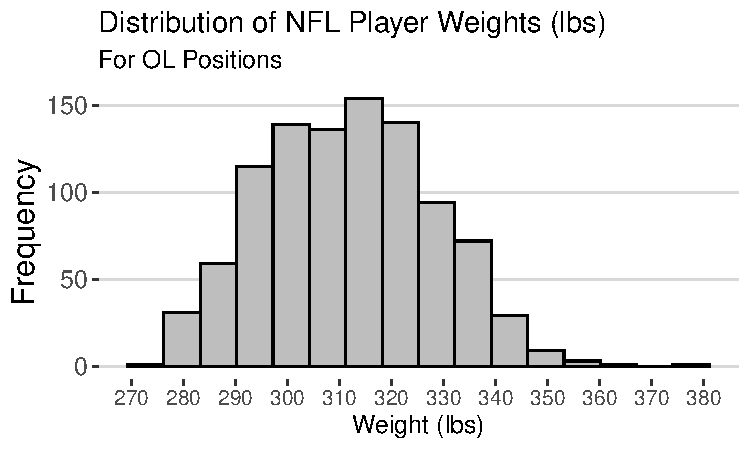
\includegraphics{Exam_1_Version_A_files/figure-latex/unnamed-chunk-2-1.pdf}

\begin{enumerate}
\item[3pts (a)]{What proportion of players weigh more than 327 lbs?}
\item[]
\item[]
\item[]
\item[]
\item[3pts (b)]{What proportion of players weigh between 293 lbs and 327 lbs?}
\item[]
\item[]
\item[]
\item[]
\item[5pts (c)]{Aaron Brewer, an offensive lineman for the Tennesee Titans, weighs 274.8 lbs. Using the $\pm 2s$ rule, is Aaron Brewer's weight an outlier relative to the rest of the NFL?}
\item[]
\item[]
\item[]
\item[]
\end{enumerate}

\newpage
\begin{enumerate}
\item[8pts \bf 13.)]{Each of the following distributions has a mean of either $\mu = 60$ or $\mu = 100$, and a standard deviation of either $\sigma = 10$ or $\sigma = 25$. Label each distribution with its mean and standard deviation.}
\end{enumerate}

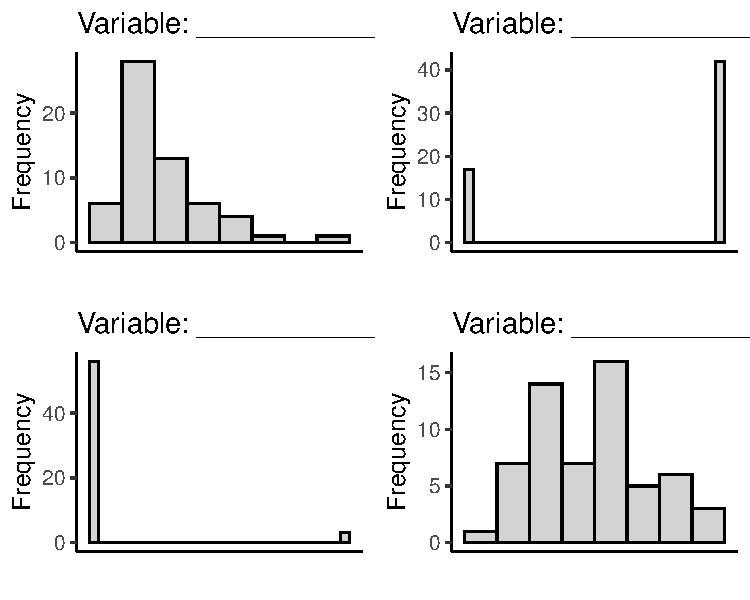
\includegraphics{Exam_1_Version_A_files/figure-latex/unnamed-chunk-3-1.pdf}

\newpage
\begin{enumerate}
\item[8pts \bf 12.)]{Describe the shape of the following distributions and for each distribution identify if the mean will be larger, smaller or the same as the median.}
\end{enumerate}

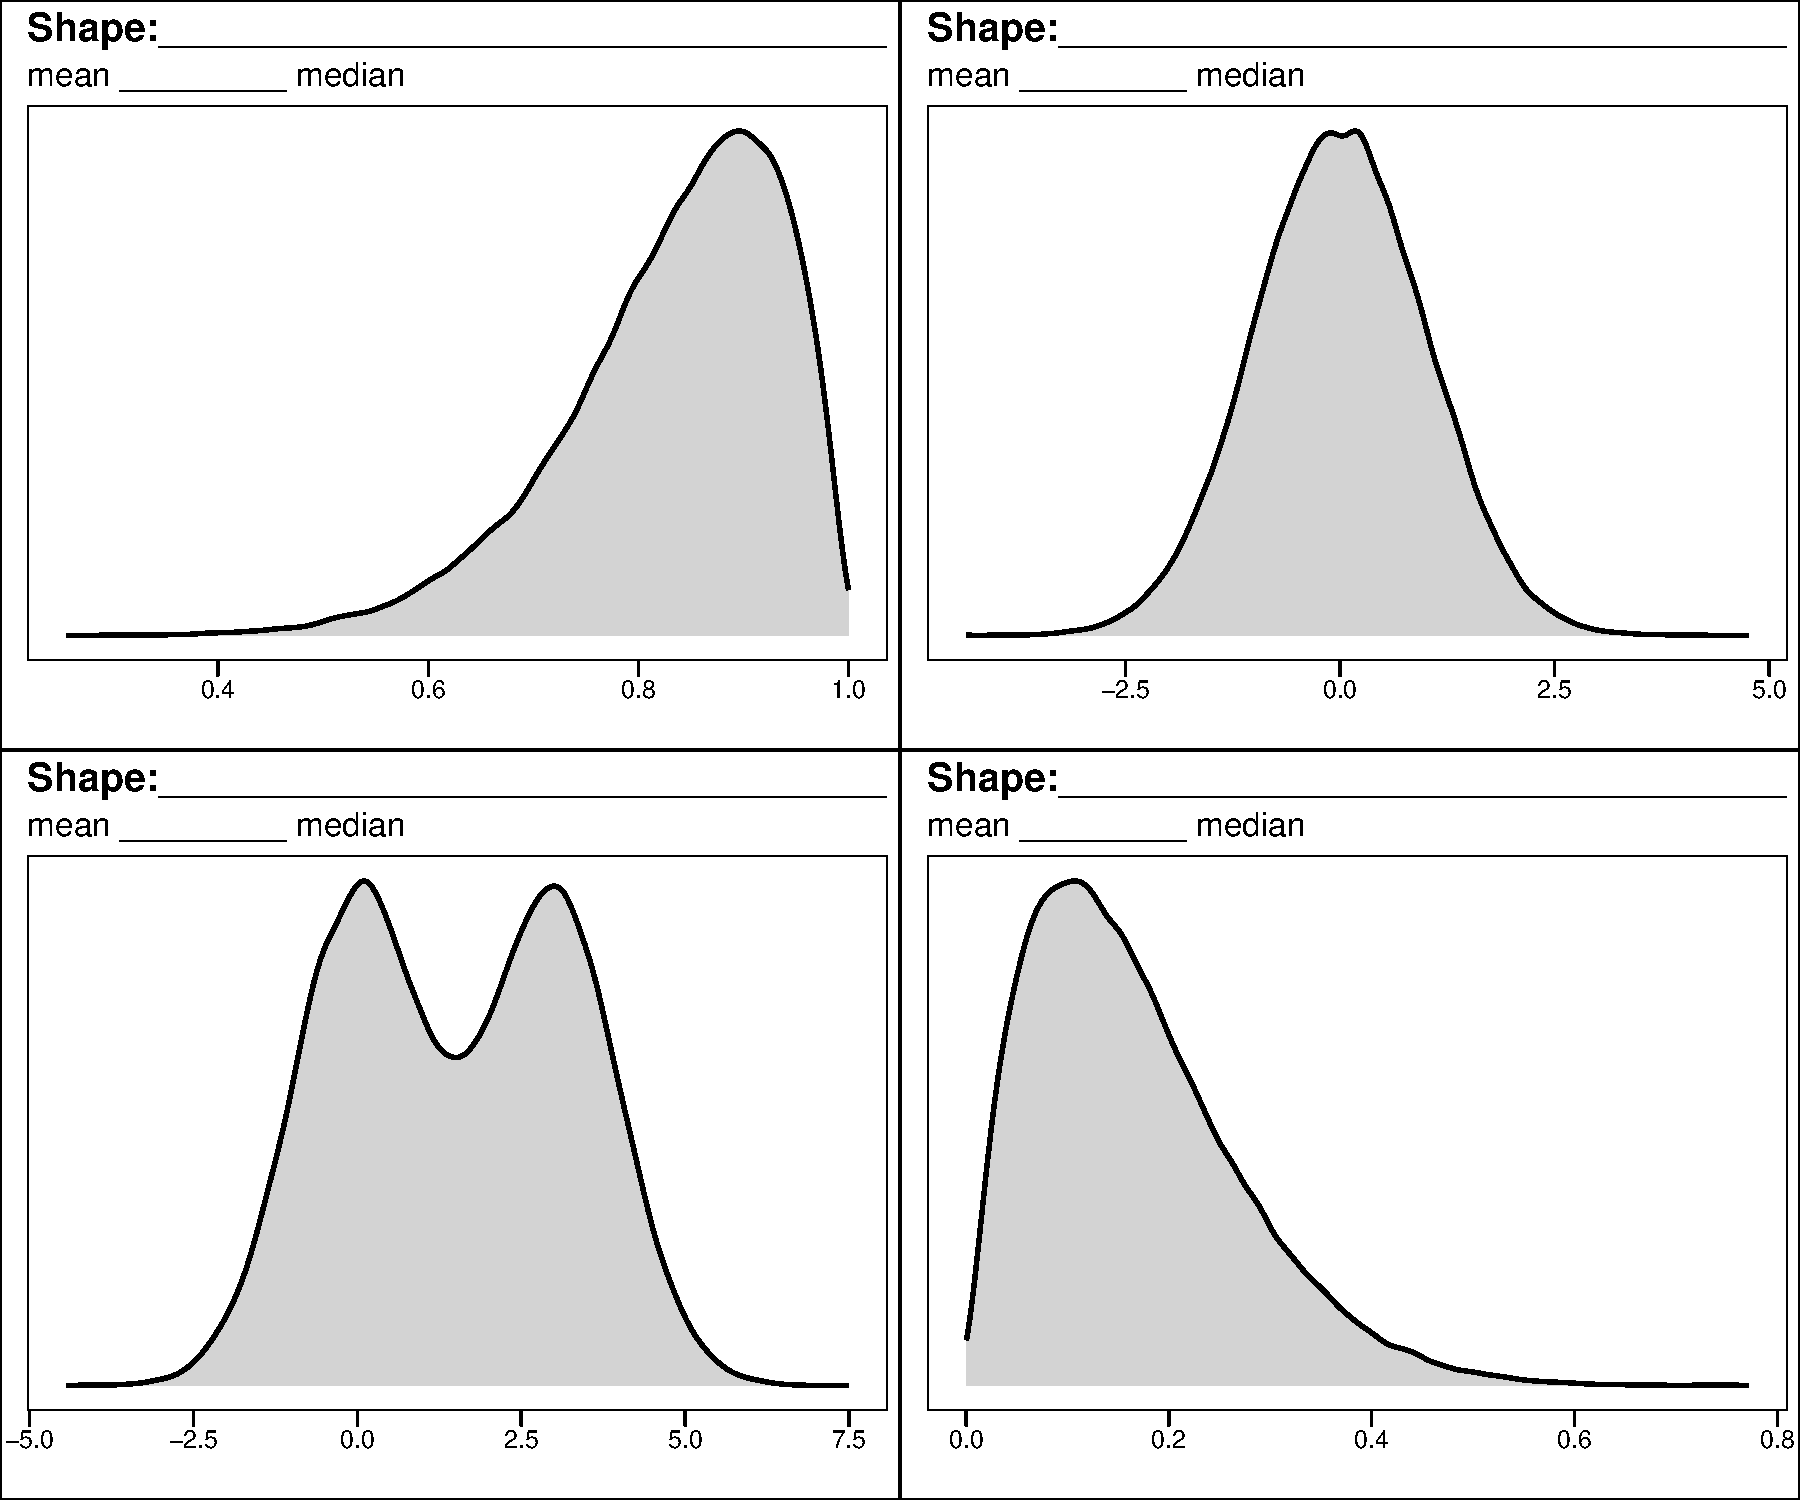
\includegraphics{Exam_1_Version_A_files/figure-latex/unnamed-chunk-4-1.pdf}

\newpage
\begin{enumerate}
\item[18pts \bf 14.)] \textbf{Table 1.} gives the distribution of a quantitative variable $x$. Use this table to answer parts (a) and (b)
\end{enumerate}

\begin{table}

\caption{\label{tab:unnamed-chunk-5}}
\centering
\begin{tabular}[t]{rrrr}
\toprule
X & Frequency(X) & Relative Frequency(x) & Cumulative Relative Fequency\\
\midrule
5 & 8 & 0.133 & 0.133\\
6 & 5 & 0.083 & 0.217\\
7 & 2 & 0.033 & 0.250\\
8 & 15 & 0.250 & 0.500\\
9 & 7 & 0.117 & 0.617\\
\addlinespace
10 & 8 & 0.133 & 0.750\\
11 & 5 & 0.083 & 0.833\\
12 & 10 & 0.167 & 1.000\\
\bottomrule
\end{tabular}
\end{table}

\begin{enumerate}
\item[9pts (a)]{Plot the cumulative distribution and use this plot to find the $25th$, $50th$, and $75th$ percentiles}
\end{enumerate}

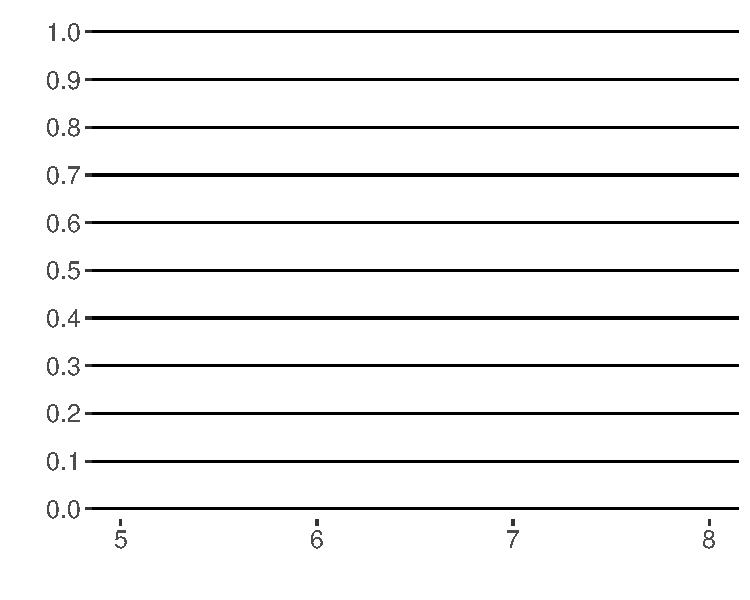
\includegraphics{Exam_1_Version_A_files/figure-latex/unnamed-chunk-6-1.pdf}

\(25th = \_\_\_\_\) \(50th = \_\_\_\_\) \(75th = \_\_\_\_\)

\newpage
\begin{enumerate}
\item[9pts (b)] Below is a box and whisker plot for the frequency table in \textbf{table 1}. Using the relevant statistics, label the values of the minimum, maximum, Q1, Q3, and IQR [hint you can use your calculations from part (a)]. 
\end{enumerate}

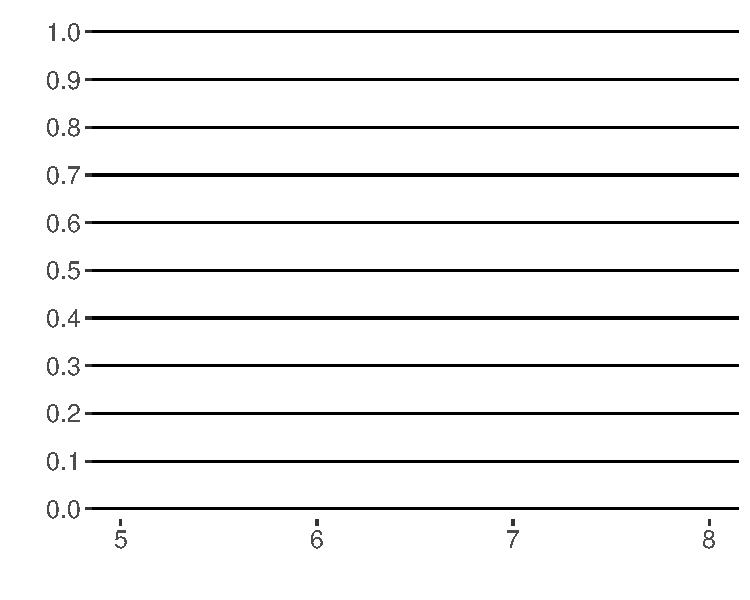
\includegraphics{Exam_1_Version_A_files/figure-latex/unnamed-chunk-7-1.pdf}

\begin{enumerate}
\item[ 4pts \bf(bonus)]{Why is the sample variance divided by $n-1$ instead of $n$ like the sample mean? explain you answer (a mathematical demonstration can also help)}
\end{enumerate}

\end{document}
